\subsection{Estudo geométrico}
O estudo geométrico é uma avaliação simples de alcance dos manipuladores
industriais no ambiente do aro câmara. Tem como objetivo verificar se o
manipulador, assumindo diferentes posições de base, consegue alcançar
todos os pontos da pá dentro das restrições da tarefa HVOF. O estudo leva em
consideração as seguintes posições para o manipulador: escotilha superior e base
móvel; manipulador em frente à pá e base móvel verticalmente; manipulador entre
as pás e base móvel verticalmente. 

Assumimos $R = 3.95 m$ e $R_m = 3 m$, onde $R$ é a distância do centro do cone à
superfície do aro câmara, e $R_m$ é o comprimento da pá. Dado isso, podemos
inferir o comprimento do aro câmara $P = 2*\pi *R = 24.81 m$ e, como são quatro
pás, são $4*R_m = 12 m$ cobertos por pás e $P-4*R_m = 12.81 m$ simetricamente
distribuídos entre as pás. Em relação ao centro do cone, o setor circular que
cada pá ocupa tem um ângulo de $\alpha = \frac{R_m*2*\pi}{P} = 0.76$, e setor
circular entre pás com ângulo $\beta = \pi/4$. A
figura~\ref{pa} mostra os parâmetros acima.

\begin{figure}[h!]
\centering
	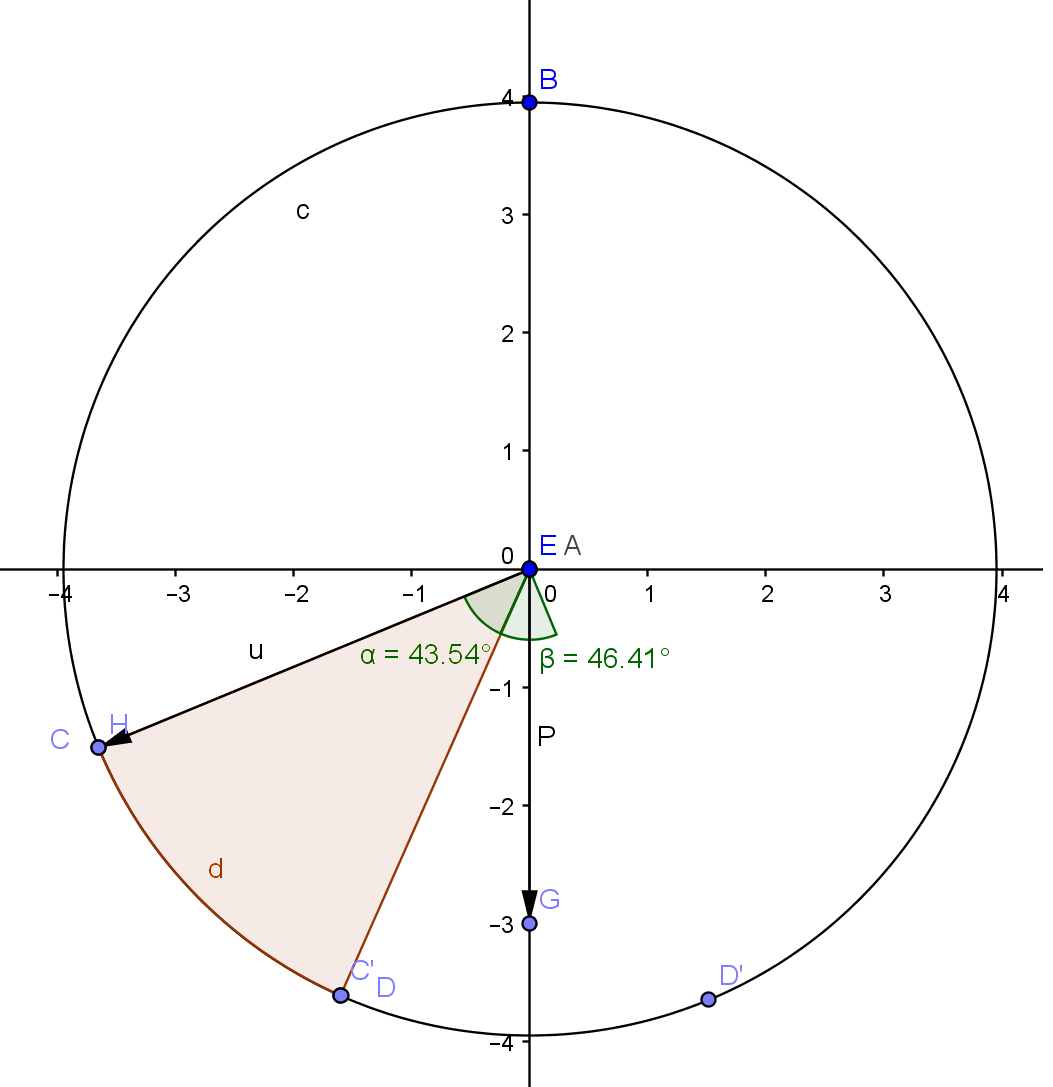
\includegraphics[width=\columnwidth]{figs/estudo/geometrico/pa.png} 
	\caption{Parâmetros do aro câmara.}
	\label{pa}
\end{figure}

Utilizando notação vetorial, temos: $\overrightarrow{P} = (0,-R,0)$. Considere
$$\overrightarrow{\widetilde{P}} = R_z(-(\alpha/2 + \beta/2))
\overrightarrow{P}$$, onde $R_z$ é rotação em  torno de $Z$. Logo
$$\overrightarrow{\widetilde{P}} = (-R sin(\alpha/2 + \beta/2),-R cos(\alpha/2 +
\beta/2),0)$$,  e o vetor $$\overrightarrow{d} = R_{\overrightarrow{\overline{\widetilde{P}}}}(-\omega)R_z(\alpha/ +
\beta/2)\overrightarrow{P}$$, onde 
$R_{\overrightarrow{\overline{\widetilde{P}}}}$ é rotação em torno do vetor
unitário $\overrightarrow{\overline{\widetilde{P}}}$ e $\omega$ é o ângulo de
rotação da pá em seu próprio eixo (valor que pode variar de $0$ a $28^o$).
Dessa forma, busca-se o $$min (\left \| \overrightarrow{d} - \overrightarrow{M} 
\right \|) =\left \| R_{\overrightarrow{\overline{\widetilde{P}}}}(-\omega)R_z(\alpha/ +
\beta/2)\overrightarrow{P} - \overrightarrow{M} \right \|$$, onde
$\overrightarrow{M}=(0,x,0)$ é a localização da base do manipulador. Dessa
forma, obtemos a menor distância entre base e o extremo da pá para $\omega,
x, \beta$. Consequentemente, pode-se inferir o alcance mínimo do manipulador.

Os valores de $\beta$ alteram a localização da base fixa em relação à pá,
simulando a rotação da pá da turbina. Para $\beta = 0$, por exemplo, o
manipulador se encontra em frente à pá e para $\beta = \pi/4$ ele está entre as
pás.

Na escotilha superior, como há restrição em relação ao manipulador (LBR 820), há
a necessidade de base móvel, que pode assumir diversos comprimentos e posições.
A solução de uma base com dois elos está representada na figura
